\section{Conclusion of Problem Analysis}

During the research for this project, we have decided on what technologies we will use for solving the problem stated in the W-diagram \ref{fig:wdiagram}.

We will use a rover with multiple sensors to navigate around in a set environment. This rover will produce a 2D map of its surroundings, with the possibility of implementing equipment for 3D mapping. We will use both sound and light sensors for navigation and mapping. Ultrasonic-sensors will be used for close encounter manoeuvres for their high precision at a close range (up to 4m)\cite{hcsr40datesheet} and a optical flow sensor will be used to measure the distance travelled. For mapping we will be using a laser sensor, that will either automatically turn 360$^{\circ}$ or we will implement a motor to rotate the sensor.

The rover will both be remote controlled and autonomous for navigation. For reference points we will use the optical flow sensor, located on the bottom of the vehicle to help determine our current location and the distance travelled from the starting location.

The control computer will be a Raspberry Pi running an optimized version of the Debian Linux operating system, called Raspbian. On top of the operating system, we will install the ROS (Robot Operating System) framework, which provides libraries and tools to help software developers create robot applications\cite{ros}.
The reason for using the Raspberry Pi is that it can multi-task, read many sensors at the same time and build the 2D map on the go. Whereas for other microcontrollers, like the Arduino, we would only be able to collect data and need to build the map from it later, using another computer.

\begin{figure}[H]
	\centering
	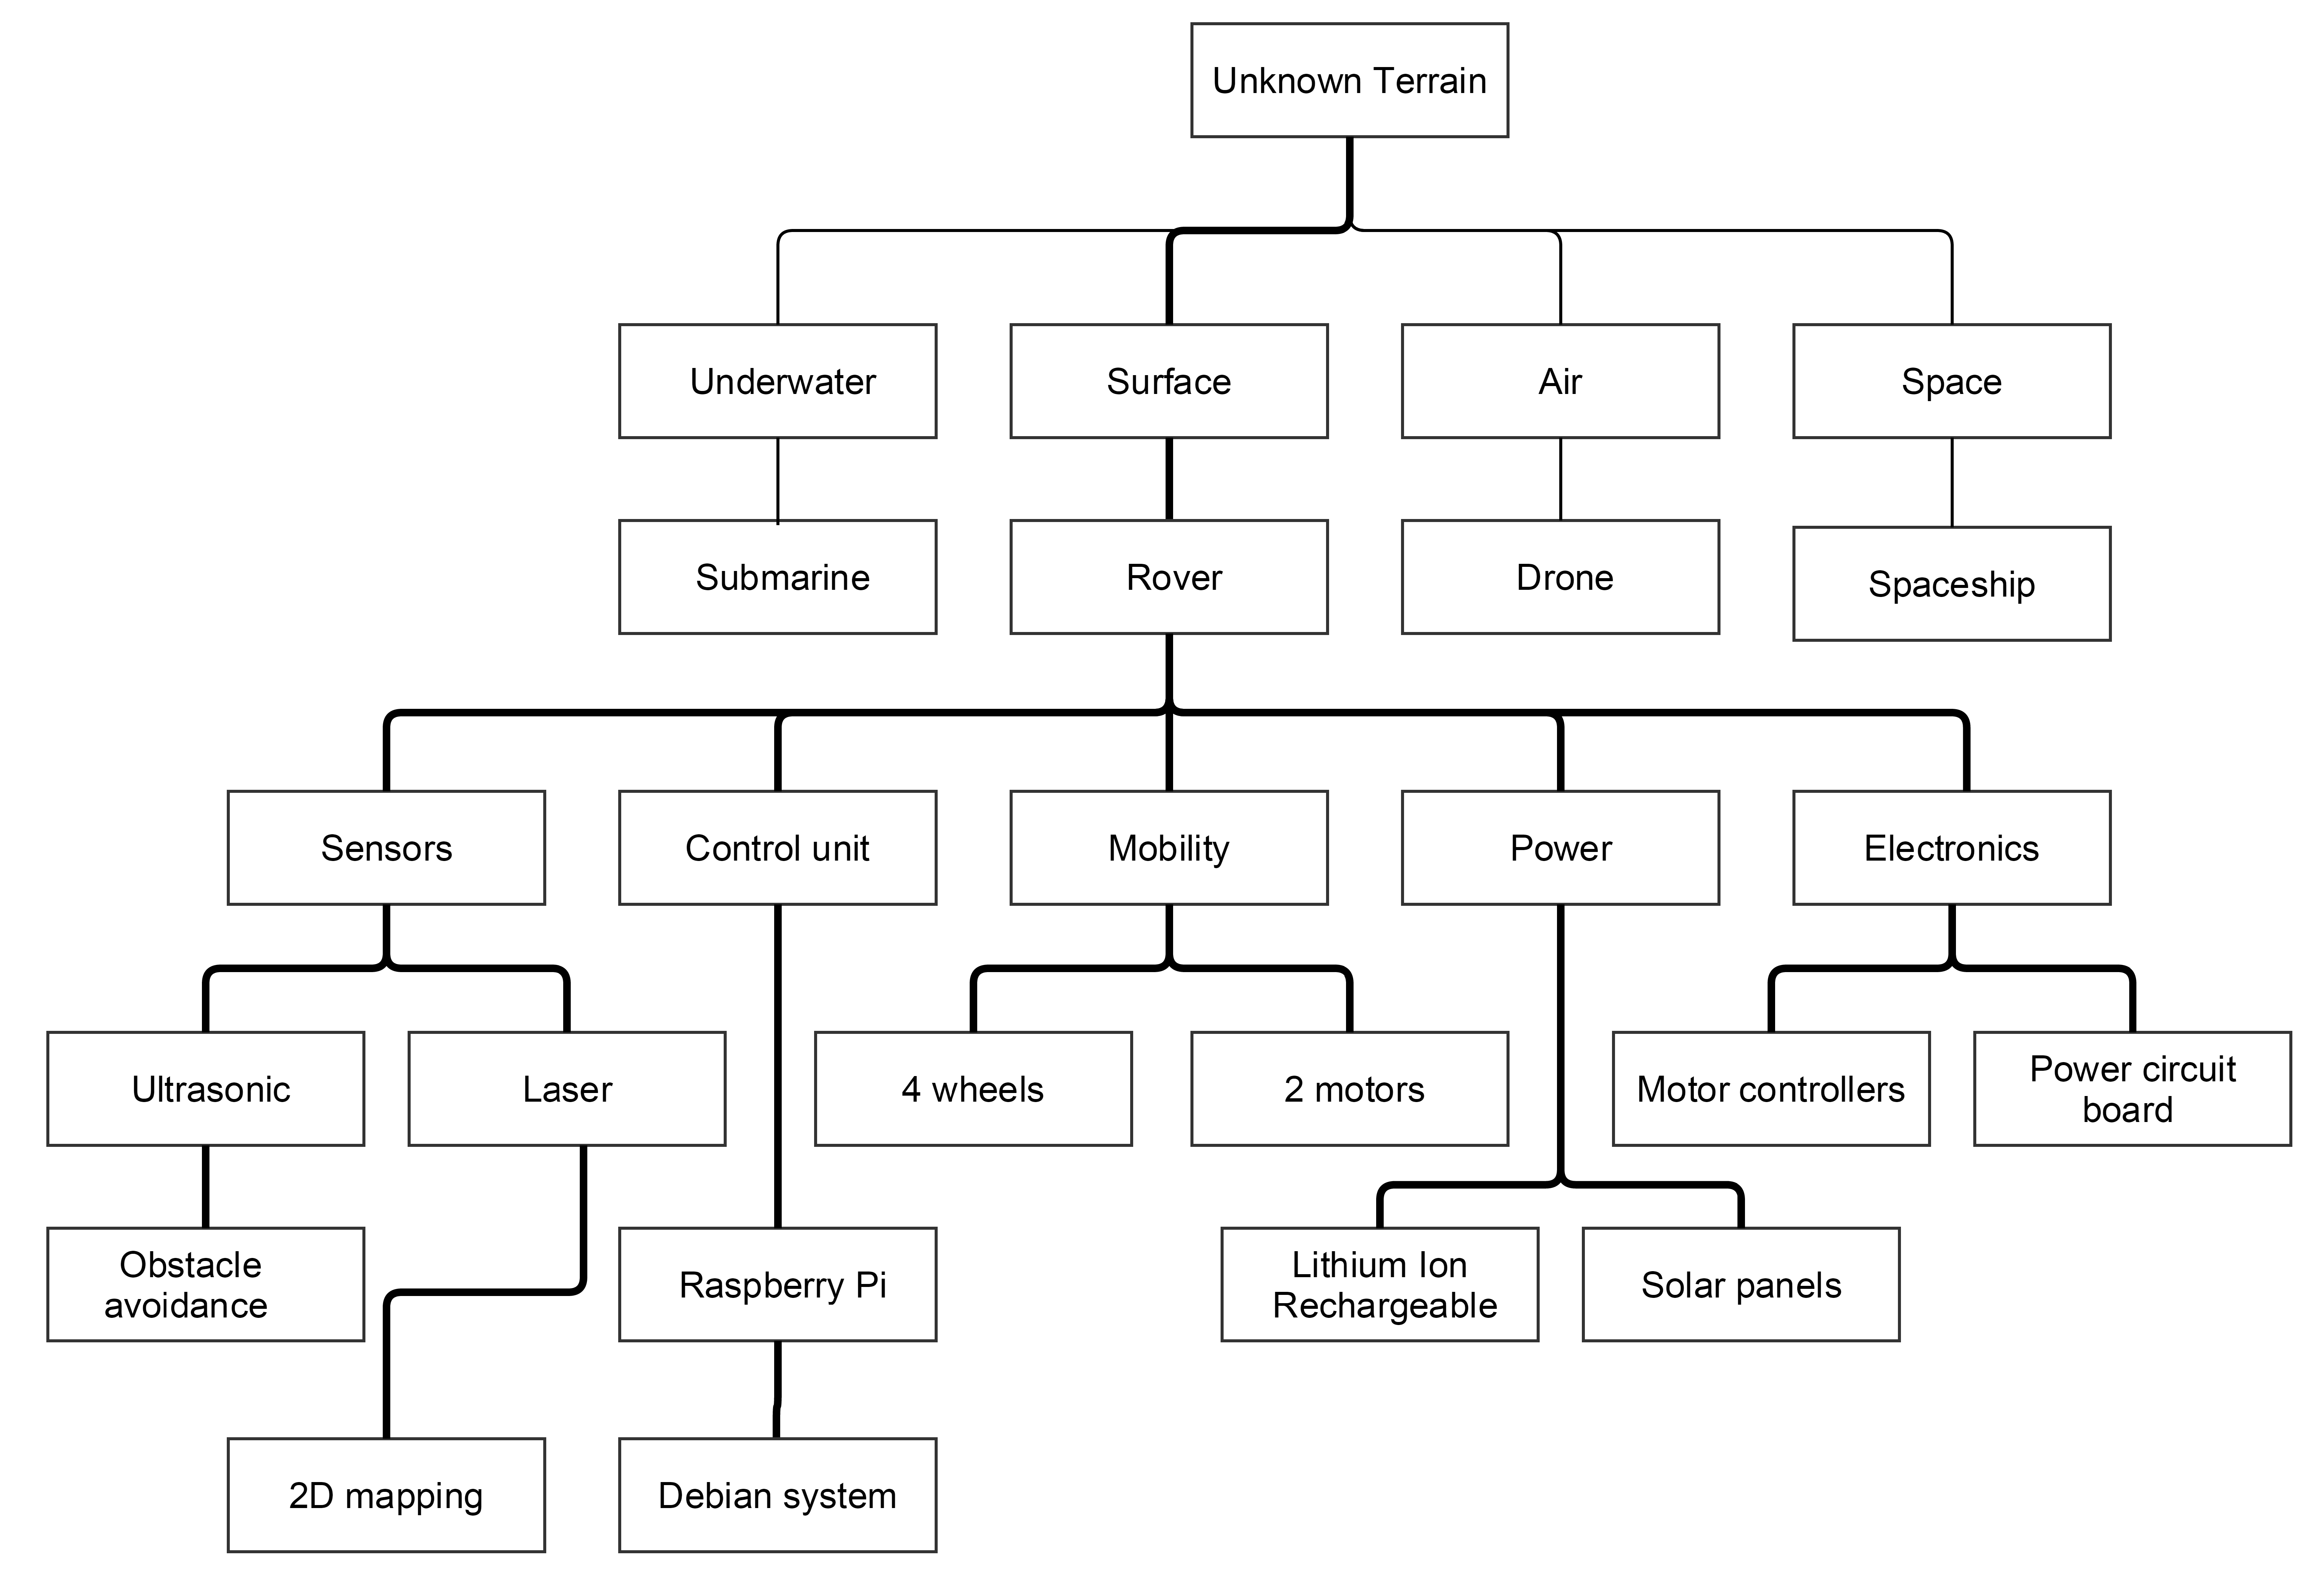
\includegraphics[scale=.1]{images/level3.png}
	\caption{Flowchart of the prototype idea.}
	\label{fig:level3}
\end{figure}

This picture shows how the flowchart from chapter one was expanded. We decided to focus on rovers, and extended the prototype requirements accordingly.

\clearpage
